% vim: set spelllang=fr:
\chapter{Introduction}
\label{ch:intro}

\section{Objectifs}

\subsection{L'annotation en rôles sémantiques}

L'annotation en rôles sémantiques est une tâche d'analyse sémantique aux
applications nombreuses, telles que l'extraction et la recherche d'information,
la traduction automatique, ou encore le résumé automatique de textes.

Elle répond à la question « Qui a fait Quoi à Qui, Comment, Où et Quand ? ».
Prenons pour exemple la phrase \emph{Mrs. Aouda essaya vainement de retenir Mr.
Fogg} (extrait du \emph{Tour du monde en quatre-vingts jours} de Jules Verne).
L'annotation en rôles sémantique déterminera que la phrase correspond à une
situation de tentative (grâce à la présence du verbe « essayer »), puis
déterminera parmi les syntagmes liés aux verbes quel est l'Agent, l'Activité
tentée, et le Résultat (\emph{vainement}). Ainsi, le résultat de l'annotation
serait :

\begin{figure}[ht]
    \centering
    \begin{tabular}{cccc}
    [Agent]  & \textbf{Tentative} & [Résultat]  & [Activité]         \tabularnewline
    Mrs. Aouda & \textbf{essaya}  & vainement & de retenir Mr. Fogg. \tabularnewline
    \end{tabular}
    \caption{\label{fig:introsrl}Le verbe \emph{essayer} déclenche la situation \emph{Tentative}.
    Les différents syntagmes liés au verbe jouent chacun un rôle sémantique.}
\end{figure}

% TODO définir frame

Différents informations sont disponibles après l'annotation en rôles sémantiques.

\begin{itemize}
    \item Le prédicat ayant déclenché la frame est identifié. Dans la
        figure~\ref{fig:introsrl}, c'est un verbe, mais d'autres parties du
        discours peuvent déclencher une frame.
    \item La frame est identifiée, ici \emph{Tentative}.
    \item Enfin, les rôles exprimés sont annotés. Par exemple, \emph{Mrs.
        Aouda} est l'Agent.
\end{itemize}

\subsection{Applications}

Selon \cite{gildea2002automatic}, l'annotation en rôles sémantiques est une
évolution naturelle de certains travaux sur l'extraction d'information où les
systèmes traitent des situations très spécifiques, par exemple la détection de
résultats d'évènements sportifs ou la détection dans des corpus journalistiques
de l'acquisition d'entreprises. En effet, à chaque nouveau système d'extraction
d'information dans un domaine différent, il est nécessaire de redéfinir les
différents patrons sémantiques et d'entraîner un nouveau système sur de
nouvelles données. En s'appuyant sur le corpus FrameNet et pour évoluer vers
une généralisation de ces systèmes, \cite{gildea2002automatic} présentent le
premier système général d'annotation en rôles sémantiques. Sans pour autant
remplacer les systèmes d'extraction d'information\footnote{TODO différences},
l'annotation en rôles sémantiques a été utilisée dans diverses applications,
notamment les systèmes de questions-réponses \citep{shen2007using},
l'extraction d'évènements \citep{exner2011using},  l'analyse d'opinions
\citep{das2012structure} ou la traduction automatique
\citep{bazrafshan2013semantic}. Un des intérêts de la généralité de
l'annotation en rôles sémantiques est de ne pas être limitée aux tâches les
plus classiques en Traitement Automatique des Langues. Ainsi, l'annotation en
rôles sémantiques à été utilisée pour la détection de plagiat
\citep{osman2012improved}, la prédiction des cours de bourses
\citep{xie2013semantic}, la génération de scènes 3D \citep{chang2014semantic},
ou l'interprétation de recettes de cuisine \citep{malmaud2014cooking}.

\subsection{Contraintes}

% TODO intégrer à LIMA et le dire :)
Nous souhaitons que notre système d'annotation en rôles sémantiques puisse être
utilisé dans un environnement industriel dans lequel d'une part l'annotation en
rôles sémantiques n'est pas l'objectif principal et d'autre part les domaines à
couvrir ne sont pas connus à l'avance. Ces contraintes majeures en découlent.

\paragraph{Cadre ouvert} Se contenter de désambiguïser certains mots ou se
limiter à un domaine fermé n'est pas satisfaisant ici. Les inventaires de sens
utilisés doivent couvrir l'ensemble des sens présents dans une langue. La
contrainte de traiter l'ensemble des verbes du vocabulaire est ici plus
importante que de pouvoir traiter les noms, adjectifs et adverbes.

\paragraph{Langue française} Le français dispose d'un nombre limité de
ressources sémantiques en cadre ouvert. Il n'existe pas aujourd'hui de VerbNet,
WordNet ou de FrameNet du français avec une couverture et une qualité proche de
leurs équivalents respectifs en langue anglaise. Ne disposant pas des moyens
pour créer de telles ressources manuellement, le système présenté doit pouvoir
se contenter de transpositions automatiques de ces ressources vers le français.
Cette approche de mutualisation des ressources au niveau de la langue doit
permettre une adaptation de ces travaux à d'autres langues que l'anglais et le
français, même si ce n'est pas l'objet de cette thèse.

\paragraph{Simplicité} Nous voulons que notre système soit très simple à mettre
en place et qu'il soit tout aussi facile de corriger quelques erreurs
spécifiques, même au prix d'une performance moins bonne que des approches plus
complexes dans le cas général. La stratégie que nous adoptons est de simplifier
nos systèmes, et des les améliorer une fois qu'ils ont montré leurs limites.

\paragraph{Efficacité} Cette contrainte est moins forte que les autres, mais
reste nécessaire pour que les solutions présentées puissent être utilisées à
large échelle. L'annotation en rôles sémantiques est un problème difficile de
classification automatique et certains systèmes ont des temps d'entraînement et
d'exécution trop longs pour l'utilisation que nous voulons en faire ici.

\section{Objectifs}
\label{objectifs_these}

% TAL a besoin d'infos sur les verbes, c'est difficile et fragile, et on a
% besoin d'énormes corpus
Le Traitement Automatique des Langues requiert des lexiques et de larges
quantités de données annotées pour analyser efficacement des textes dans le
domaine général. Obtenir cette quantité de données est un problème en soi connu
sous le nom de "knowledge acquisition bottleneck" en désambiguïsation lexicale
\citep{gale1992using}. Annoter de plus en plus de données de manière efficace
réduira ce problème pour certains domaines, mais d'autres stratégies sont
nécessaires pour atteindre nos objectifs dans plus de domaines. Une possibilité
est d'utiliser au mieux les données annotées en perfectionnant les algorithmes
existants, une autre est d'utiliser intelligemment les données non annotées qui
existent en quantité bien plus importante. Une troisième possibilité, celle que
nous choisissons, est d'encoder les lexiques de manière efficiente pour couvrir
une large partie du vocabulaire. C'est ce qui est fait par exemple dans VerbNet
où les traits partagés par les mêmes verbes sont explicitement notés, ce qui
permet à chaque modification dans VerbNet de mieux traiter un certain nombre de
verbes au lieu d'un seul.

% VerbNet a montré son efficacité dans le domaine de par son approche
% pragmatique. Vient des classes de Levin, donne des correspondances entre
% syntaxe et sémantique
Deux difficultés majeures qu'affrontent les créateurs de lexique sont la
granularité de sens et la distinction des sens. Ces deux difficultés sont
gérées par les classes de Levin \citep{levin1993english}. Dans ces classes, les
verbes sont classifiés principalement à travers leur alternances syntaxiques,
ce qui fournit un critère qui est à la fois facilement observable et qui
produit des distinctions sémantiques intéressantes. VerbNet
\citep{kipperschuler2005verbnet} est un lexique électronique basé sur les
classes de Levin. Il encode non plus les alternances mais les cadres de
sous-catégorisation valables pour chaque classe, et rajoute des informations de
rôle et de sémantique à travers une logique des prédicats simplifiée. De
nouvelles classes, constructions et verbes ont étés ajoutés à VerbNet au fil
des ans. Au-delà de son encodage efficace, VerbNet est un lexique adapté au
Traitement Automatique des Langues : on peut utiliser un cadre de
sous-catégorisation pour mapper des syntagmes à des rôles thématiques
\citep{swier2005exploiting,pradet2013revisiting}. Grâce à sa couverture élevées
(plus de quatre mille verbes distincts) et son groupement de verbes utile,
VerbNet est bien adapté à l'annotation en rôles sémantiques.

% TODO De la même manière, WordNet ...

% Dans les langues autres que l'anglais, cette ressource utile n'existe pas
% mais ne demande qu'à exister étant donné le potentiel \textit{cross-lingual}
% de VerbNet. Il y a souvent des ressources proches, moins utiles, plus
% linguistiques, existent.
Cependant, un VerbNet et un WordNet de qualité n'existent pour le moment que
pour l'anglais. De telles ressources serait pourtant encore plus utile pour les
langues moins ressourcées où les corpus annotés en rôles sémantiques n'existent
pas. VerbNet a un potentiel inter-linguistique, visible notamment avec le
portuguais \citep[section 2.2.2]{kipperschuler2005verbnet}. Adapter VerbNet
vers une nouvelle langue suffisamment proche de l'anglais permet de conserver
sa structure, ainsi que l'information sémantique et les rôles thématiques, ce
qui donne la possibilité de produire un lexique utile sans des années de
travail manuel.

% En particulier, en français, les tables du LADL décrivent le comportement
% syntaxique des verbes et le LVF découpe les verbes du français
% sémantiquement. Un certain nombre de difficultés empêche d'utiliser ces
% ressources en TAL
% TODO le dire, mais où ?

L'objectif de cette thèse est donc de fournir les \emph{ressources} nécessaires
en traduisant WordNet et VerbNet (Partie~\ref{part:translation}) et
\emph{méthodes} (Partie~\ref{part:srl}) répondant à ces objectifs.

\section{Ressources lexicales utilisées}

\subsection{WordNet}
\label{presentation_wordnet}

La première ressource lexicale à tirer partie de la possibilité de représenter
le lexique sous la forme d'un graphe est WordNet, dont l'élaboration a commencé
en 1985 \citep{miller1990introduction}. Établi sur des principes
psycholinguistiques, WordNet propose quatre graphes pour les quatre parties du
discours formant une classe ouverte : noms, verbes, adjectifs, adverbes. Les
nœuds du graphe sont des ensembles de synonymes (\emph{synonym sets} ou
\emph{synsets}). Un synset regroupe plusieurs mots, une définition, et
potentiellement des exemples.

% TODO placement des figures une fois le texte un peu plus stable

\begin{figure}[t]
    \centering
    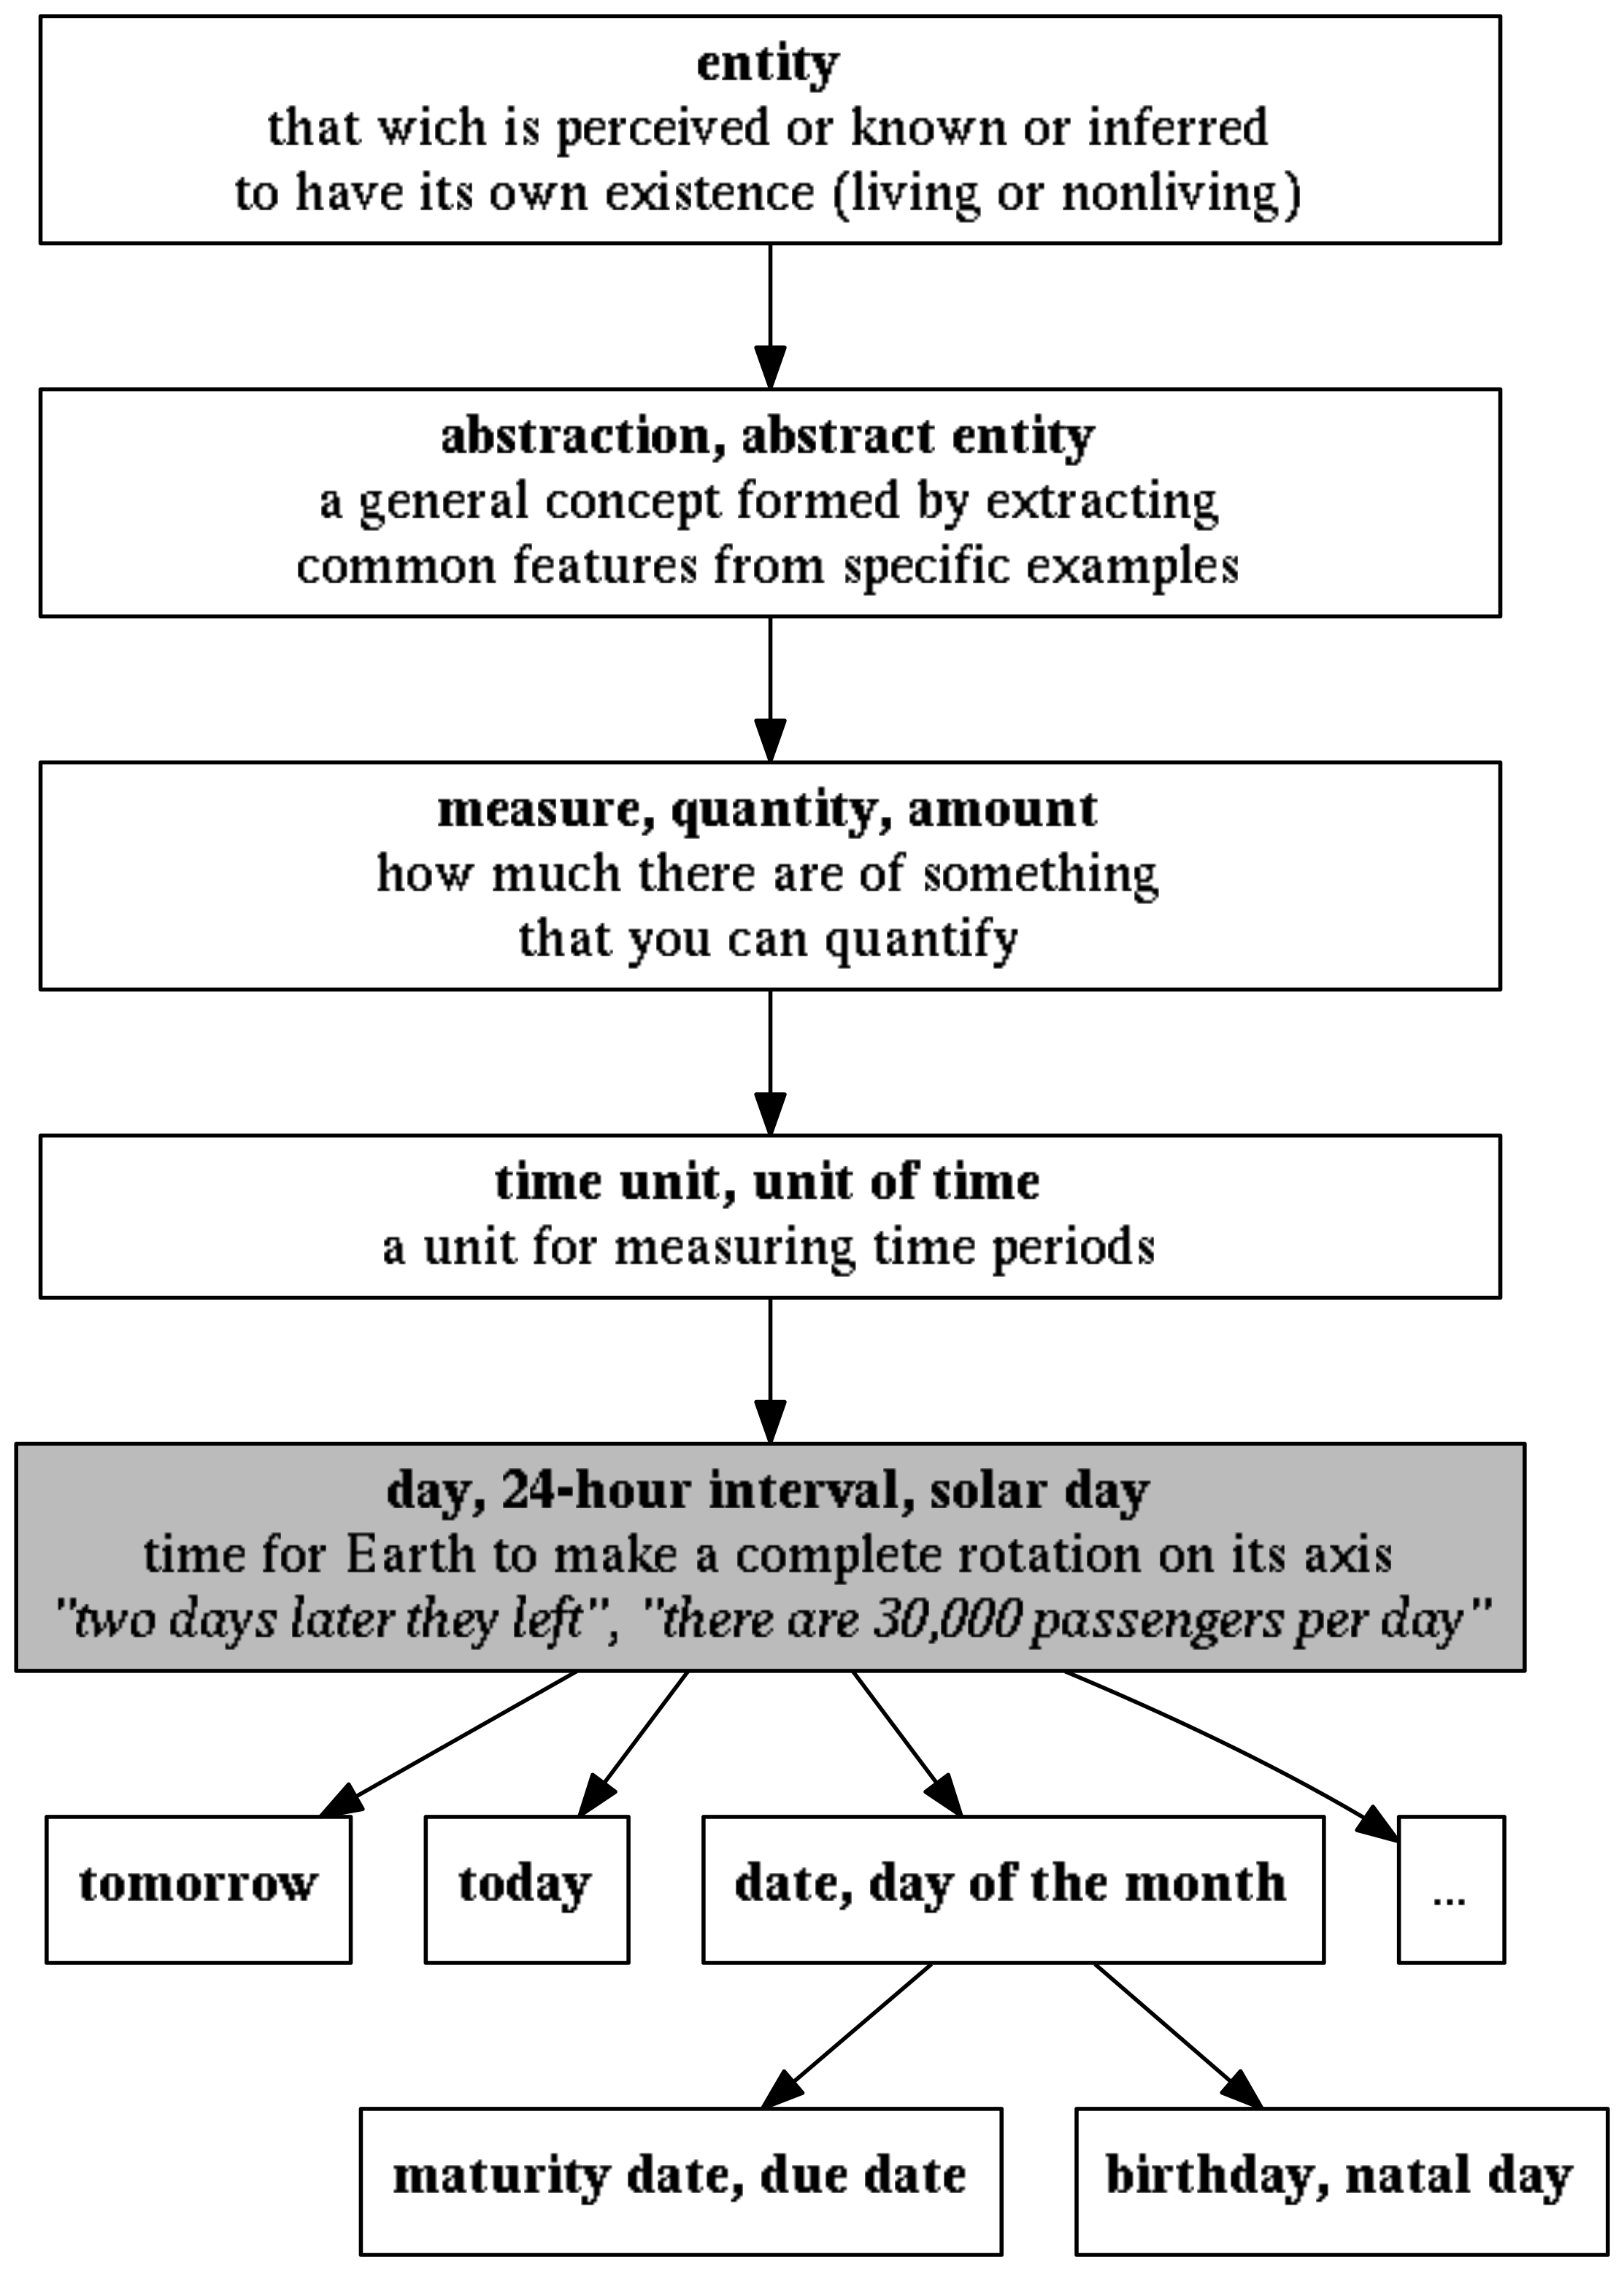
\includegraphics[width=0.6\textwidth]{fig/wordnet_hypernymy.png}
    \caption{\label{fig:wordnet_hypernymy}Hypéronymie dans WordNet autour du
        synset \emph{day}. Les synsets au-dessus de \emph{day} sont ses hypéronymes
        (\emph{day} est-un \emph{time unit}), et les synsets au-dessus font partie de
        ses hyponymes (\emph{tomorrow} est-un \emph{day}).}
\end{figure}

Chaque synset est lié à d'autres synsets à travers un certain nombre de
relations telles que l'hypéronymie, la méronymie de partie (\emph{guidon} est
un méronyme de partie de \emph{vélo}), l'antonymie, etc. Si on ne considère que
l'hypéronymie, WordNet peut être visualisé comme un arbre
(Figure~\ref{fig:wordnet_hypernymy}). En considérant les autres relations,
WordNet est un graphe (Figure~\ref{fig:wordnet_relations}).

\begin{figure}[t]
    \centering
    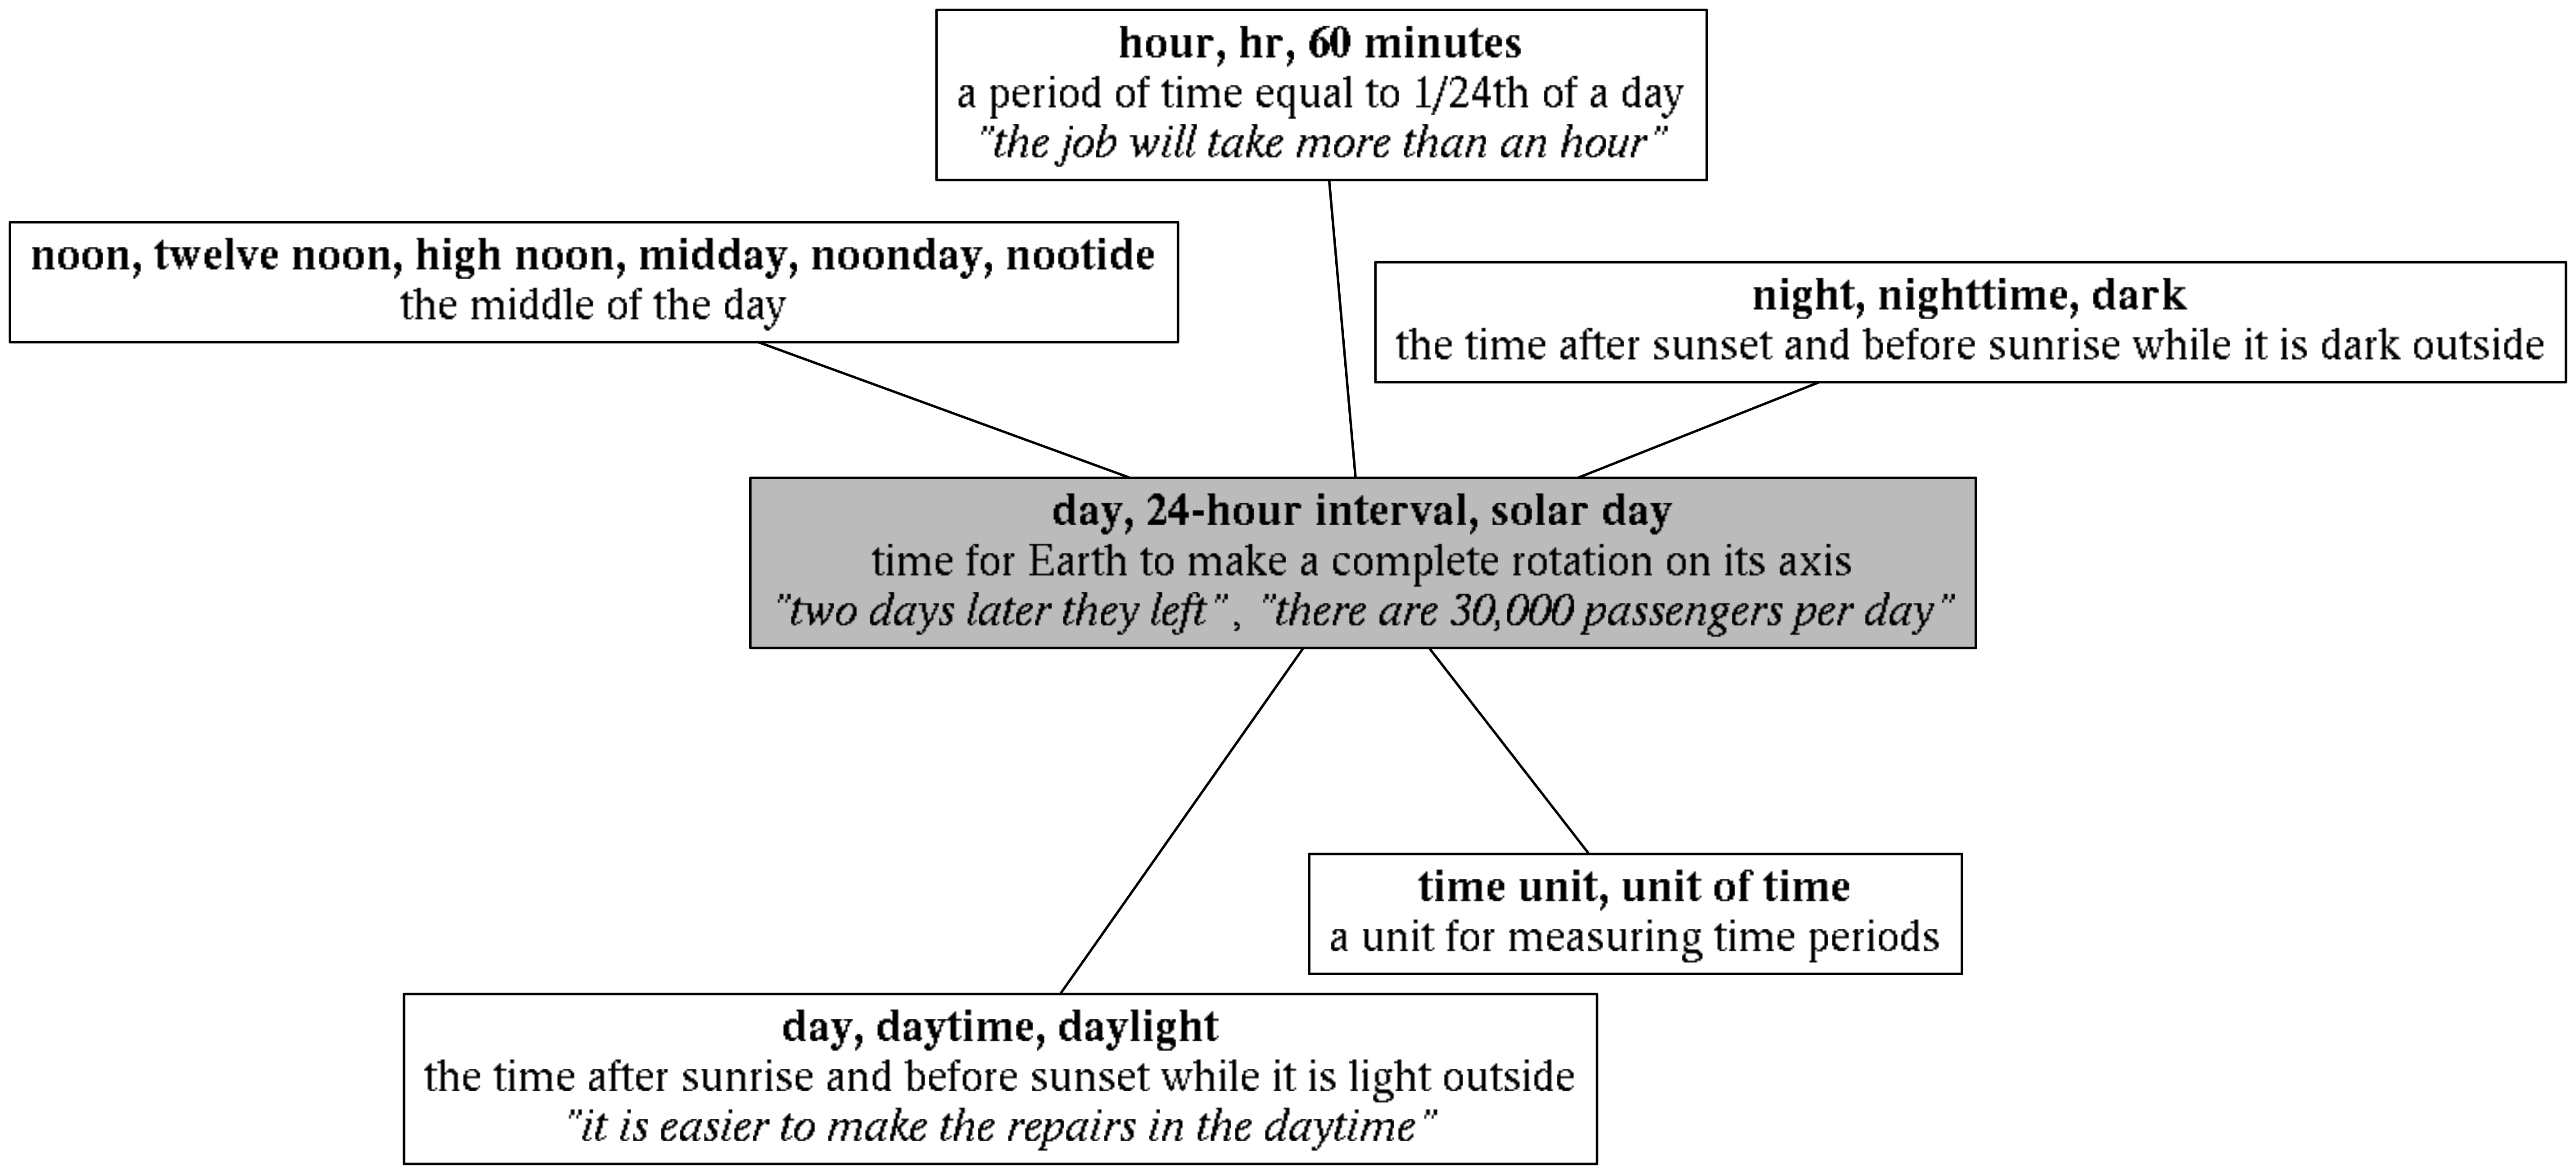
\includegraphics[width=0.7\textwidth]{fig/wordnet_relations.png}
    \caption{\label{fig:wordnet_relations} Le synset \emph{day} est aussi lié à
        d'autres synsets si on considère d'autres relations que l'hypéronymie et
        l'hyponymie.}
\end{figure}

% TODO cite bond survey
Les sens proposés ont étés utilisés pour annoter différents corpus dont le
corpus SemCor, ce qui a permis d'entraîner des systèmes supervisés. WordNet est
rapidement devenu le standard de la désambiguïsation lexicale et a été utilisé
dans de nombreuses campagnes d'évaluation \citep{navigli2009word}. C'est aussi
une ressource très utilisée de manière générale dans le domaine du Traitement
Automatique des Langues\footnote{Au moment de l'écriture de ce manuscrit, ses
10~000 citations sur Google Scholar sont le meilleur moyen de l'attester.}.

\subsection{Les classes de Levin}

\cite{levin1993english} est une classification des verbes anglais établie
suivant un principe simple : le comportement syntaxique des verbes détermine en
partie leur sens. Après avoir défini un certain nombre d'alternances de
diathèses possibles, les verbes sont classés en groupes partageant les mêmes
alternances.

% TODO exemple d'alternance venant vraiment de Levin.

Cette classification a trois intérêts pour l'annotation en rôles sémantiques :

\begin{itemize}

    \item Une grande majorité des verbes anglais sont couverts, rendant la
        ressource utile pour des annotations à large échelle.

    \item La classification est hiérarchique et regroupe de nombreux verbes :
        avec une cinquantaine de classes principales, des généralisations et
        partages d'informations entre les verbes de classes identiques ou
        proches sont possibles.

    \item Les comportements syntaxiques déterminent les comportements
        sémantiques, ce qui correspond au schéma classique de l'annotation en
        rôles sémantiques qui s'appuie sur une analyse syntaxique.

\end{itemize}

%\subsection{Intersection des classes de Levin}

% TODO raccourcir sans dire de bêtises

Dans les classes de Levin, toute distinction de classe doit s'appuyer sur un
critère clairement observable, tel que le comportement syntaxique ou les
propriétés morphologiques d'un verbe. Et ceci même si la distinction entre deux
classes est motivée par la volonté de prendre en compte une différence
sémantique entre deux groupes de verbes.

Pour cette raison, les groupements de verbes sont parfois grossiers d'un point
de vue sémantique. Ainsi, dans les \textit{put verbs} se trouve la classe
\textit{Pocket} qui regroupe les verbes "mettre dans sa poche" (\emph{put}) et
"mettre en prison" (\emph{jail}). Cependant, le comportement syntaxique est le
même : le regroupement est logique et les différences de sens ne sont a priori
pas gênantes pour des tâches telles que l'annotation en rôles sémantiques qui
ne se basent pas sur le sens précis des verbes. Il est possible d'affiner
automatiquement les classes de Levin en réalisant des intersections de classes
: les verbes obtenues seront alors définis plus strictement
\citep{dang1998investigating}. Cette possibilité n'est cependant pas utilisée
dans nos travaux.

\subsection{VerbNet}
\label{subsec:presentation_verbnet}

VerbNet \citep{kipperschuler2005verbnet} est à la fois une version électronique
et une version améliorée des classes de Levin, qui se retrouvent améliorées sur
plusieurs fronts :

\begin{itemize}

    \item de nouvelles classes provenant de \cite{korhonen2004extended}
        intégrant les verbes acceptant des complétives, mais aussi des
        syntagmes adjectivaux et adverbiaux ou encore des particules.

    \item de nouveaux verbes provenant de \cite{dorr2001lcs} ont étés intégrés

    \item les verbes ont étés liés à WordNet, OntoNotes, PropBank et FrameNet
        \citep{palmer2009semlink}

    \item de nombreuses corrections ont étés apportées au fil des versions. Une
        des améliorations prévues dans le futur est de tirer du Sketch Engine
        pour ajouter d'autres verbes. \citep{bonial2013expanding}.

\end{itemize}

Ces améliorations ont à la fois contribué à VerbNet en largeur (nouvelles
classes) et en profondeur (nouveaux verbes, nouvelles constructions
syntaxiques). La base de données continue d'évoluer, la dernière version prévue
au moment de l'écriture de ce manuscrit étant la 3.2.4.

VerbNet contient 3769 lemmes, 5257 entrées réparties en 500 sous-classes dont
270 classes de niveau 2 et 109 classes de niveau 1. La hiérarchie relativement
plate. Pour chaque (sous-)classe, ce lexique indique :

\begin{itemize}
        \item la liste des verbes de la classe,
        \item les rôles thématiques en jeu ainsi que leur restrictions de sélection,
        \item la liste des \emph{frames} VerbNet.
\end{itemize}

Une frame inclut une phrase d'exemple, une formule syntaxique donnant la
liaison entre les syntagmes et les rôles thématiques, une formule sémantique
basée sur la logique des prédicats explicitant la relation entre les
participants et les évènements.

% TODO exemple

% TODO autre exemple non intuitif avec verbe complet en bas

% TODO Introduire fig:example_srl
 VerbNet a montré la cohérence de sa classification et est très
utilisé, notamment pour l'annotation en rôles sémantiques
\citep{swier2005exploiting,palmer2013semantic} où il présente l'intérêt de ne
pas être restreint à un domaine spécifique tout en couvrant une large partie
des occurrences des verbes anglais dans un texte donné.

\begin{figure}[ht]
    \centering
    \begin{tabular}{ccc}
        \toprule
        Carol & crushed   & the ice \\
        Agent & V         & Patient \\
        \midrule
        The ice & crushes & easily  \\
        Patient & V       &         \\
        \bottomrule
    \end{tabular}
    \caption{\label{fig:example_srl}Ces deux phrases annotées avec la classe VerbNet carve-21.2 mettent en évidence que la position des arguments ne détermine pas directement les rôles: le sens et la voix de \textit{crush} ne change pas mais l'annotation sémantique est différente.}
\end{figure}

\subsection{Les Verbes Français et Lexique-Grammaire}

À partir des années 70 deux ressources lexicales pour les verbes français ont
été dévelopées : LVF et LG\footnote{Plus tard, dans les années 1990, une autre
ressource a été dévelopée : Dicovalence. Nous ne l'utilisons presque pas dans
nos travaux.}. Pourquoi ne pas utiliser ces ressources directement ? Un des
intérêts des classes de Levin et de VerbNet par rapport aux ressources
françaises est leur approche pragmatique qui se traduit notamment par l'absence
de prise en compte des emplois métaphorique d'un verbe donné. Ainsi, les tables
du LADL incluent des usages tels que \textit{L'idée gallopait dans son esprit}
qui peuvent induire en erreur une application. Certains usages métaphoriques
peuvent certes être prise en compte dans VerbNet, mais ils n'y sont pas par
défaut. En effet, \cite{brown2012semantic} proposent une analyse systématique
des emplois métaphorique de deux verbes représentatifs et montrent qu'utiliser
VerbNet pour raisonner sur les emplois métaphorique d'un texte est en partie
possible au prix d'une complexité plus importante et de prédicats sémantiques
moins précis.

% TODO mieux que sous-sous-sous et nombre de E2f.1
LVF (Les Verbes Français, \cite{dubois1997verbes}) contient environ 25000
entrées classées en 14 classes sémantiques, 54 sous-classes
syntactico-sémantiques, 248 sous-sous-classes et XXX sous-sous-sous-classes.

% TODO exemple

LG (Lexique-Grammaire, \cite{gross1975methodes,boons1976structure}) comporte
lui 14 000 entrées classifiées en 67 «~tables~», chaque table groupant des
verbes partageant la même propriété définitoire syntaxique et potentiellement
une sémantique similaire. Chaque colonne de la table encode des restrictions
supplémentaires s'appliquant à certains des verbes de la table.

% TODO exemple


Les classes LVF et les tables LG peuvent toutes les deux être comparées aux
classes VerbNet. Cependant, ces (vieilles) ressources n'encodent ni les rôles
thématiques ni les formules sémantiques \footnote{Les notions de rôles
thématiques et d'évènement n'étaient pas répandues dans les années 1970.}.
C'est la raison principale pour laquelle nous voulons construire une nouvelle
ressource française, \verbenet{}\footnote{Le nom vient de la prononciation à la
    française qui "rajoute" un e. Le $\ni$ est simplement là pour bien marquer
ce e et ainsi essayer d'éviter la confusion avec VerbNet}. Cette ressource tire
profit d'une part des ressources existantes pour le français avec un encodage
sémantique et syntaxique riche, et d'autre part de l'information sémantique
présente dans VerbNet pour l'anglais, une langue proche du français.
